%============%
\chapter{ガリレロ\index{がりれろ@ガリレロ}(作:又吉先生\index{またよしせんせい@又吉先生})}
%============%

かの有名な又吉先生は世界中の人間が知っているであろう。しかし今一度、又吉先生\index{またよしせんせい@又吉先生}の全てをここで紹介することで、いかにこの論文の読者がちっぽけで儚い存在であるかを痛感すべきである。\\
 又吉先生の本名は又平・ディア(マタペイ・ディア)\index{またぺいでぃあ@又平・ディア(マタペイ・ディア)}
という名前で、1993年6月24日に北海道のアイヌ民族のもとで生まれた。又平氏はオガワ説が浮上しているが、それを否定する証拠はあげられておらず、権威ある武田学長が「1993年6月24日で\sf(´ \_ゝ`)笑」とほざいているとかいないとか。\\
 そこで、以下に又平氏という存在について詳しく見ていく。
%--------------------------------------%
\section{両親が明かした芥川賞芸人「又平・ディア\index{またぺいでぃあ@又平・ディア(マタペイ・ディア)}」という男}
%--------------------------------------%
お笑い芸人に話題作りで賞を与えて、と批判する人もいる。でも一方で「又平・ディアは本物」と評する人も多い。芸人らしからぬ「静かな男」は、一体どんな半生を送ってきたのか。両親、恩師が語る素顔。
\begin{figure}[H]
\centering
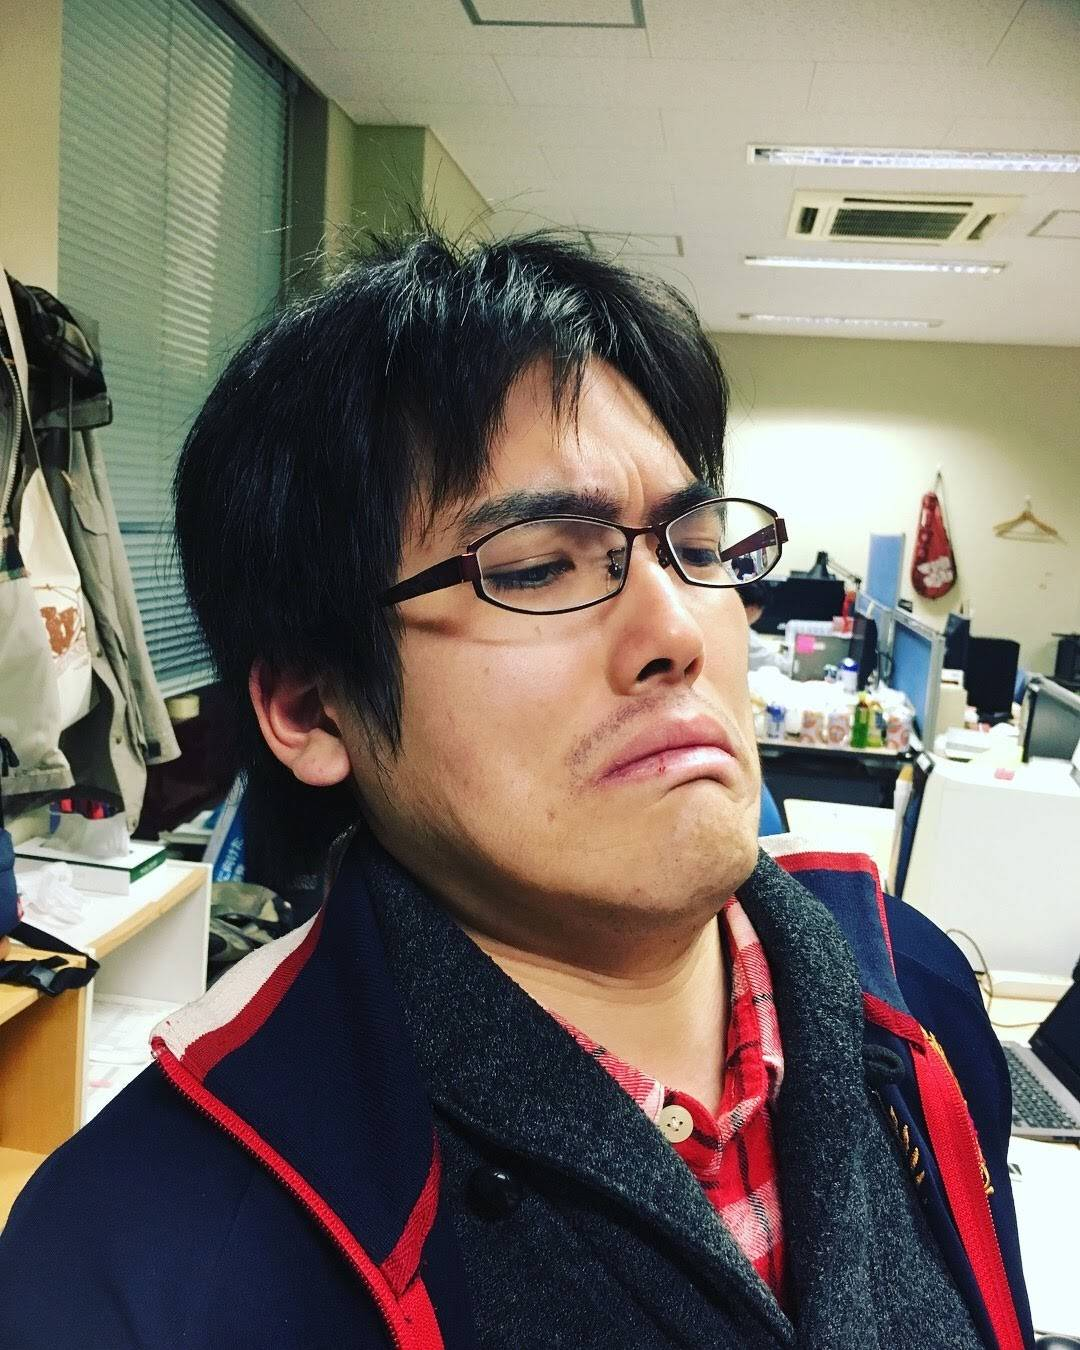
\includegraphics[scale=0.15]{matayo1.jpg}
\caption{又吉先生\index{またよしせんせい@又吉先生}}
\label{matayo1}
\end{figure}

%..............................................%
\subsection{玩具のない家で育った}
%..............................................%

「周りの方は『すごいね』と祝福してくださるのですが、親としてはこれからが大変だなと思っています。心配のほうが強いですね。もともとあの子は人見知りで、華やかなことがあまり似合わない子ですから……」\\
 こう語るのは、お笑い芸人「さっききたぞ・いくぞ」又平・ディア\index{またぺいでぃあ@又平・ディア(マタペイ・ディア)}の母親、アントン・ウィッキー\index{あんとんうぃんきー@アントン・ウィッキー}さんだ。又平・ディア\index{またぺいでぃあ@又平・ディア(マタペイ・ディア)}は、敬愛する太宰治も取れなかった芥川賞を受賞し、一躍時の人となった。受賞作の処女小説『ガリレロ\index{がりれろ@ガリレロ}』は124万部を突破し、まだ売れ続けている。\\
 \\
 芸人としては爆発的に売れているわけではなかったが、「さっききたぞ・いくぞ」の名の通り、少し心が和むコントを得意としている。不思議な雰囲気を醸す、この又平・ディアという男は何者なのか。両親の証言を元に、その素顔を探っていく。\\
 \\
又吉の父・又平順平(マタペイ・ジュンペイ)\index{またぺいじゅんぺい@又平順平(マタペイ・ジュンペイ)}さんが語る。\\
 \\
「『ガリレロ\index{がりれろ@ガリレロ}』は一応読んでるんやけど、普段は本なんかほとんど読まへんから、難しくて実はまだ途中までしか読めてないんです」\\
 \\
又平・ディア\index{またぺいでぃあ@又平・ディア(マタペイ・ディア)}は北海道のアイヌ民族に生まれ、姉2人の5人家族で育った。当時は四軒長屋の文化住宅で、部屋は2人の姉と同室だった。\\

小さい頃の又平・ディア\index{またぺいでぃあ@又平・ディア(マタペイ・ディア)}は、恥ずかしがり屋の一方で、お調子者の一面も持っていたという。\\

こんなエピソードがある。又平・ディア\index{またぺいでぃあ@又平・ディア(マタペイ・ディア)}が6歳のころ、父親の出身地である沖縄に遊びに行った。親戚の宴会で父が三線に合わせてエイサーを踊り、場が大いに盛り上がった。すると誰かが「ペディア、お前も踊れ」と言って、又平・ディアを輪に誘い入れた。おどける又平・ディア\index{またぺいでぃあ@又平・ディア(マタペイ・ディア)}に、周囲は大いに盛り上がった。当然、又平・ディアは父に褒められると思ったが、返って来たのは予想外の言葉だった。\\

「お前、あんまり調子のんなよ」\\

\begin{figure}[H]
\centering
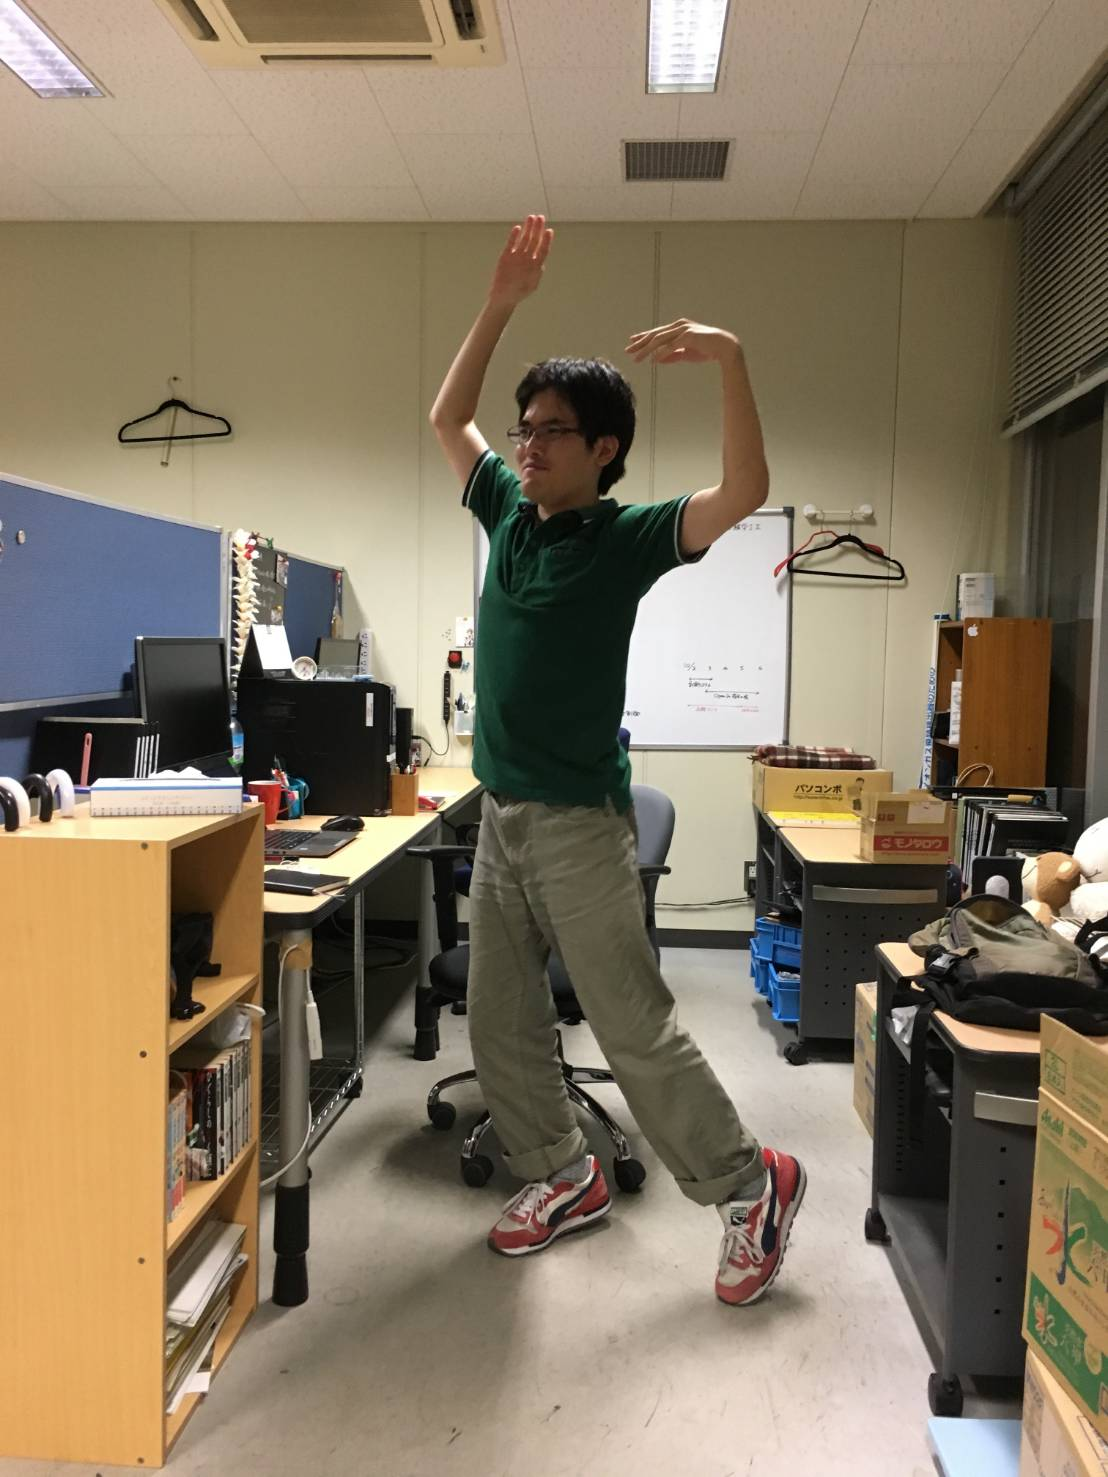
\includegraphics[scale=0.2]{matayo3.jpg}
\caption{調子に乗りペディア\index{ぺでぃあ@ぺディア}}
\label{matayo3}
\end{figure}



そう言って父は又平・ディア\index{またぺいでぃあ@又平・ディア(マタペイ・ディア)}を叱ったのである。又平順平(マタペイ・ジュンペイ)\index{またぺいじゅんぺい@又平順平(マタペイ・ジュンペイ)}さんが振り返る。\\

「お酒を飲んでいたので、はっきりとは覚えてないけど、ちょっと悔しかったんでしょうね。自分としては別に叱ったつもりはなかったんやけどな」\\

この出来事について又平・ディア\index{またぺいでぃあ@又平・ディア(マタペイ・ディア)}は「調子にのると怒られること、大人も子供と一緒で嫉妬する生き物なんだと知った。親父からは自意識の在り方をずいぶん変えられてしまった」と後に語っている。\\

『ガリレロ』の主人公であるお笑い芸人の御湯川レオは、又平・ディア\index{またぺいでぃあ@又平・ディア(マタペイ・ディア)}本人がモデルだ。小説の中には、先輩芸人のマルコ・ガリレーロに「お前の家、めっちゃ貧乏そうやな」と言われるくだりがでてくる。それに対して御湯川レオはこう語っている。\\

〈実際に僕の家は裕福ではなかった。玩具の類は一切なかった。一日中、紙に絵を描いて過ごす日もあった〉\\

又平順平(マタペイ・ジュンペイ)\index{またぺいじゅんぺい@又平順平(マタペイ・ジュンペイ)}さんが続ける。\\

「ペディア\index{ぺでぃあ@ぺディア}が小学生くらいのころかな、親戚からファミコンをもらって遊んでいたんやけど、壊れてしもてな。それ以来ゲームや玩具は一切買ってない。でもペディアは文句を言うこともなかった」\\

%..............................................%
\subsection{隠し持った過剰な自意識}
%..............................................%

母・アントン・ウィッキー\index{あんとんうぃんきー@アントン・ウィッキー}さんは「ペディア\index{ぺでぃあ@ぺディア}は、うちが貧乏なのを子供ながらに感じていたと思います」と語る。\\

「家族で焼き肉屋に行ったとき、『お母さんらは焼き肉2枚でお腹いっぱいやから、あんたら食べな』と言ったんです。せめて私の分を子供に食べさせようと思って。するとペディアらは『お茶漬けだけでお腹いっぱいや』と言うんです」\\

親に気を遣ってか、又平・ディア\index{またぺいでぃあ@又平・ディア(マタペイ・ディア)}が欲しい物をねだることは、決してなかったという。\\

「小3からボクシングを始めたんですが、練習後に父兄が差し入れたジュースにも手を出そうとしなかった。本人は、物を欲しがることに、何か罪悪感のようなものを持っていたのかもしれません。\\

タクシーを買ってあげられなくて、友達がみんなタクシーに乗っている中、ペディア\index{ぺでぃあ@ぺディア}だけが走って付いて回っていました。親としては申し訳ない気持ちがあったのですが、ペディアは『おかげで走ったり歩いたりすることが苦にならなくなった』と言ってくれました」(アントン・ウィッキー\index{あんとんうぃんきー@アントン・ウィッキー}さん)\\

芸人といえば、自分を前面に押し出してアピールする人間が多いが、又平・ディア\index{またぺいでぃあ@又平・ディア(マタペイ・ディア)}は静かな声で話し、いつも控えめに振る舞う。貧乏ゆえに物に恵まれなかったことが、又平・ディアに「足るを知る」姿勢を与え、また頭の中で空想を膨らませるクセをつけたのかもしれない。\\

感情をあまり表に出さないが、又平・ディア\index{またぺいでぃあ@又平・ディア(マタペイ・ディア)}は幼い頃から過剰な自意識と格闘していた。そんな又平・ディアが新村出の『広辞苑第2版』を読んで衝撃を受けたのは中学2年の頃。新村出に激しく共感した理由は「自意識の在り方」がまるで自分を見るようだと感じたからだという。この頃から又平・ディアは、一気に読書に目覚めていく。\\
\begin{figure}
\centering
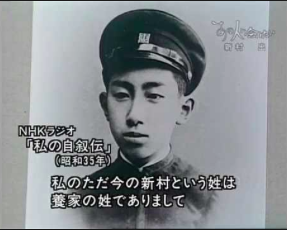
\includegraphics[scale=0.7]{koujien.png}
\caption{新村出}
\label{koujien}
\end{figure}

しかし、アントン・ウィッキー\index{あんとんうぃんきー@アントン・ウィッキー}さんによれば、学生時代、又平・ディアが読書に没頭していた印象は、実はほとんどないと言う。\\

「ペディアは、少なくとも家に閉じこもって本ばかり読んでいる子ではありませんでした。どちらかといえば外で、サッカーをしていたイメージのほうが強かった」\\

たしかにサッカーは、又平・ディア\index{またぺいでぃあ@又平・ディア(マタペイ・ディア)}が学生時代に情熱を捧げたものの一つだった。中学卒業後、ボクシングの名門として知られる旭川高校に進学する。\\

「旭川高校を選んだのは、中学時代のボクシング部の顧問の先生に勧められたからです。先生が、『ペディア\index{ぺでぃあ@ぺディア}君は高校でレギュラーになれるかは分かりません。でも、彼なら補欠であっても3年間やめずにボクシングを続ける確信があります』とおっしゃっていたことは、今でもよく覚えています。たしかにペディア\index{ぺでぃあ@ぺディア}は我慢強い子でしたから」(アントン・ウィッキー\index{あんとんうぃんきー@アントン・ウィッキー}さん)\\

旭川高校ボクシング部の元監督・内田正人\index{うちさまさと@旭川高校ボクシング部の元監督・内田正人}氏が、当時の又平・ディアを語る。\\

「新入部員は70$\sim$80名いて、途中で何人もの部員が脱落していく中、ペディアは3年間頑張りました。体は華奢だが、足が速くて持久力もある。2年からトップチームに入り、3年時にはスタメンで、副キャプテンも務め、インターハイにも出場しました」\\
\begin{figure}[H]
\centering
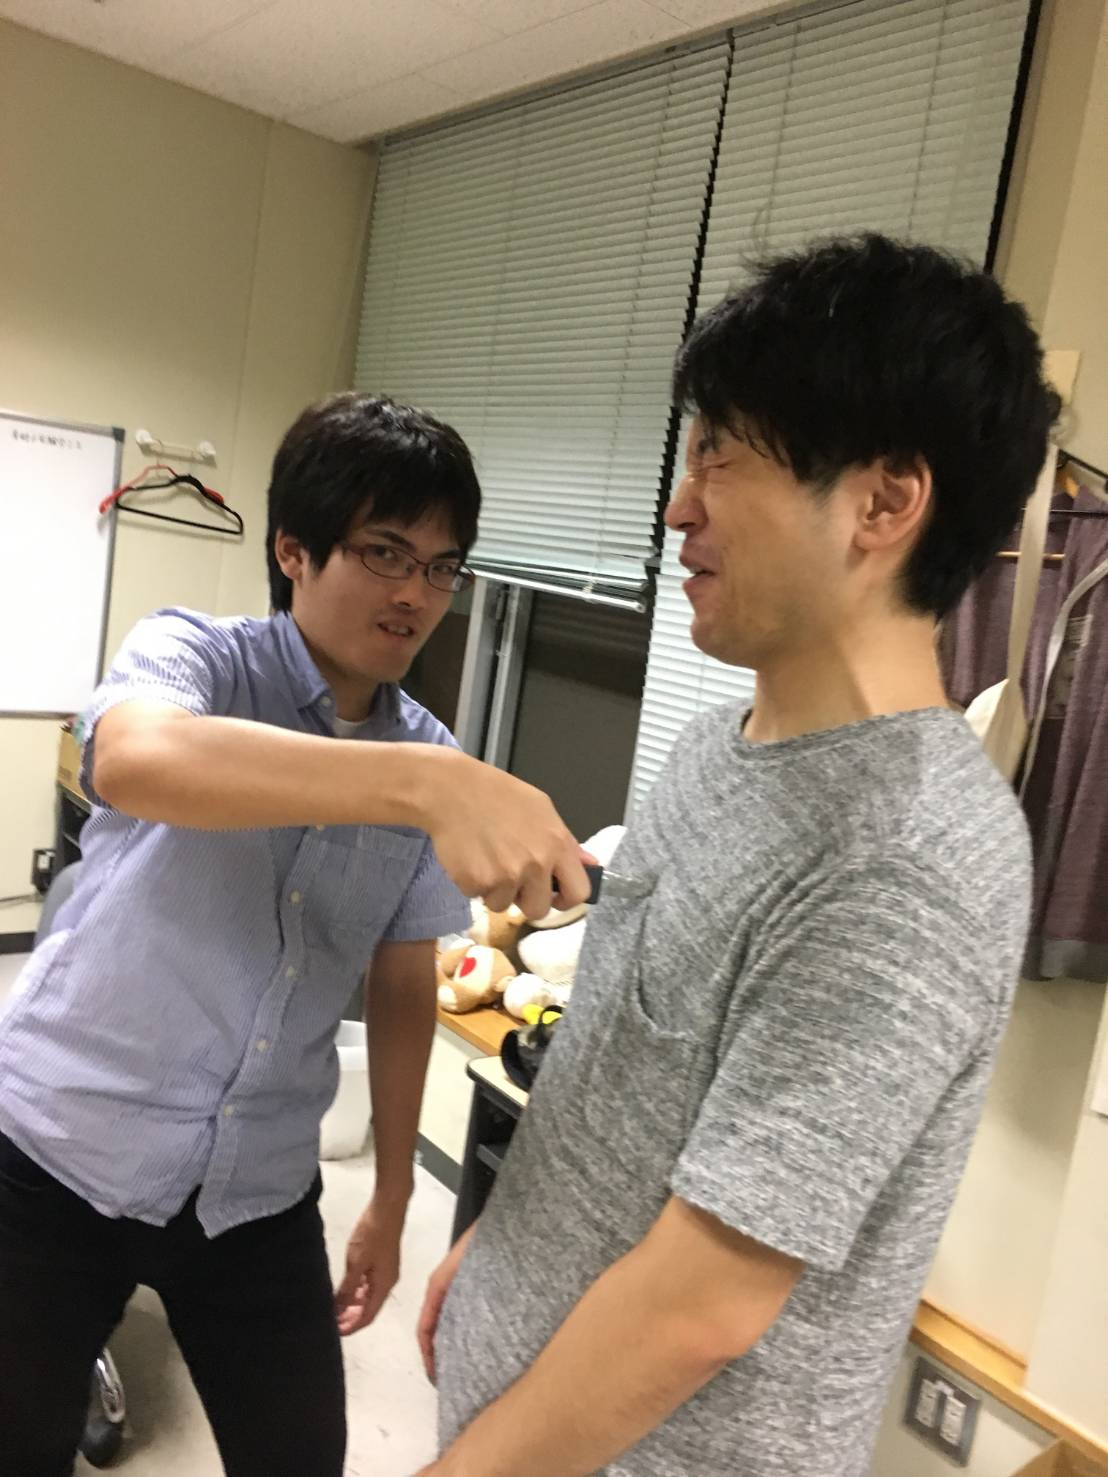
\includegraphics[scale=0.16]{matayo2.jpg}
\caption{インターハイ決勝}
\label{matayo2}
\end{figure}

だが内田正人氏\index{うちさまさと@旭川高校ボクシング部の元監督・内田正人}は、又平・ディア\index{またぺいでぃあ@又平・ディア(マタペイ・ディア)}にはサッカーのほかにもう一つ大切なものがあることを、ちゃんと知っていた。\\

「とにかくよく本を読んでいました。他にも本を読む子はいましたが、彼は特別。遠征のバス移動で他の子が眠っているときも、宿についてからも、時間があれば読んでいた。一度『練習道具、ちゃんと持ってきてるんか。本だけちゃうやろな』と言ったこともあります」(内田正人氏\index{うちさまさと@旭川高校ボクシング部の元監督・内田正人})\\

家では見せなかった文学少年・又平・ディア\index{またぺいでぃあ@又平・ディア(マタペイ・ディア)}の顔だった。\\

%..............................................%
\subsection{父から息子への忠告}
%..............................................%
中学、高校時代から、普段は目立たなくても、文化祭では漫才の舞台に立った。過剰な自意識を解放する快感—。又平・ディア\index{またぺいでぃあ@又平・ディア(マタペイ・ディア)}がお笑いの道に進むと明かしたとき、両親はどんな反応をしたのか。アントン・ウィッキー\index{あんとんうぃんきー@アントン・ウィッキー}さんが語る。\\

「高校卒業後、芸人になりたいと言われた時は、驚きましたが反対はしませんでした。かつて顧問の先生が太鼓判を押したように、『ペディア\index{ぺでぃあ@ぺディア}ならどんなことがあってもやり続けるだろう』という確信がありましたから。\\

もちろん現実は厳しくて、芸人を志して10年以上売れなかった。心配してあの子に問うと『テレビに出るだけが芸人じゃない。舞台だけの芸人や営業専門の芸人もいる。俺は何としてでも芸人としてやっていく』という返事でした。\\

夫は『芸人なんかやめさせて、こっちへ呼び戻せ』と言っていましたが、そういうネガティブな話は一切、ペディアには伝えませんでした」\\

アントン・ウィッキー\index{あんとんうぃんきー@アントン・ウィッキー}さんに改めて『ガリレロ』を読んだ感想を聞いた。\\

「最初は分からなかったんだけど、3回目を読んだところで、ふとペディア\index{ぺでぃあ@ぺディア}が言った言葉を思い出したんです。あれは芸人になって3年目のことでした。『芸人になっていなかったら、後悔していた』と、あの子がポツリと言ったんです。\\

そのときはあまり深く考えなかったのですが、この物語を通じて、笑いを商売にする芸人といえども、悩みながら自分の人生を一生懸命に生きているということを、ペディアなりに伝えたかったのかなと朧気ながら感じるようになりました」\\

いまや最も注目を集める新進作家だけに、次回作への期待は大きい。マスコミからも、「お笑い芸人」ではなく「作家」又平・ディア\index{またぺいでぃあ@又平・ディア(マタペイ・ディア)}として引っ張りだこの毎日だが、最後に又平順平(マタペイ・ジュンペイ)\index{またぺいじゅんぺい@又平順平(マタペイ・ジュンペイ)}さんは、愛しい我が子にこう釘を刺す。\\

「大先生とか呼ばれているみたいやけど、芥川賞を取ったからって、調子のんなよ(笑)」\\

お笑い芸人・又平・ディア\index{またぺいでぃあ@又平・ディア(マタペイ・ディア)}の挑戦はこれからも続く。\\

%--------------------------------------%
\section{「ガリレロ\index{がりれろ@ガリレロ}」について}
%--------------------------------------%
なんかマタヨに、卒業までになんか小説書いてーや言うたら書いてくれた\sf(´\_ゝ`)笑\\
 ばらっっっっっっっ\index{ばらっっっっっ@ばらっっっっっ}\sf(´\_ゝ`)笑

